%%%%%%%%%%%%%%%%%%%%%%%%%%%%%%%%%%%%%%%%%
% Short Sectioned Assignment
% LaTeX Template
% Version 1.0 (5/5/12)
%
% This template has been downloaded from:
% http://www.LaTeXTemplates.com
%
% Original author:
% Frits Wenneker (http://www.howtotex.com)
%
% License:
% CC BY-NC-SA 3.0 (http://creativecommons.org/licenses/by-nc-sa/3.0/)
%
%%%%%%%%%%%%%%%%%%%%%%%%%%%%%%%%%%%%%%%%%

%----------------------------------------------------------------------------------------
% PACKAGES AND OTHER DOCUMENT CONFIGURATIONS
%----------------------------------------------------------------------------------------

\documentclass[paper=a4, fontsize=11pt]{scrartcl} % A4 paper and 11pt font size

\usepackage[T1]{fontenc} % Use 8-bit encoding that has 256 glyphs
\usepackage{fourier} % Use the Adobe Utopia font for the document - comment this line to return to the LaTeX default
\usepackage[norsk]{babel} 
\usepackage[utf8]{inputenc}
\usepackage{amsmath,amsfonts,amsthm} % Math packages
\usepackage{tikz} % drawing package

\usepackage{sectsty} % Allows customizing section commands
\allsectionsfont{\centering \normalfont\scshape} % Make all sections centered, the default font and small caps

\usepackage{fancyhdr} % Custom headers and footers
\pagestyle{fancyplain} % Makes all pages in the document conform to the custom headers and footers
\fancyhead{} % No page header - if you want one, create it in the same way as the footers below
\fancyfoot[L]{} % Empty left footer
\fancyfoot[C]{} % Empty center footer
\fancyfoot[R]{\thepage} % Page numbering for right footer
\renewcommand{\headrulewidth}{0pt} % Remove header underlines
\renewcommand{\footrulewidth}{0pt} % Remove footer underlines
\setlength{\headheight}{13.6pt} % Customize the height of the header

\numberwithin{equation}{section} % Number equations within sections (i.e. 1.1, 1.2, 2.1, 2.2 instead of 1, 2, 3, 4)
\numberwithin{figure}{section} % Number figures within sections (i.e. 1.1, 1.2, 2.1, 2.2 instead of 1, 2, 3, 4)
\numberwithin{table}{section} % Number tables within sections (i.e. 1.1, 1.2, 2.1, 2.2 instead of 1, 2, 3, 4)

\setlength\parindent{0pt} % Removes all indentation from paragraphs - comment this line for an assignment with lots of text

%---- Listings --------------
\usepackage{color}
\definecolor{light-gray}{gray}{0.95}
\usepackage{listings}

\lstset{ %
language=C,                % choose the language of the code
basicstyle=\footnotesize,       % the size of the fonts that are used for the code
numbers=left,                   % where to put the line-numbers
numberstyle=\footnotesize,      % the size of the fonts that are used for the line-numbers
stepnumber=1,                   % the step between two line-numbers. If it is 1 each line will be numbered
resetmargins=true,              % reset line numbers
numbersep=5pt,                  % how far the line-numbers are from the code
backgroundcolor=\color{white},  % choose the background color. You must add \usepackage{color}
showspaces=false,               % show spaces adding particular underscores
showstringspaces=false,         % underline spaces within strings
showtabs=false,                 % show tabs within strings adding particular underscores
frame=single,           % adds a frame around the code
tabsize=2,          % sets default tabsize to 2 spaces
captionpos=b,           % sets the caption-position to bottom
breaklines=true,        % sets automatic line breaking
breakatwhitespace=false,    % sets if automatic breaks should only happen at whitespace
escapeinside={\%*}{*)}          % if you want to add a comment within your code
}

%----------------------------------------------------------------------------------------
% TITLE SECTION
%----------------------------------------------------------------------------------------

\newcommand{\horrule}[1]{\rule{\linewidth}{#1}} % Create horizontal rule command with 1 argument of height

\title{ 
\normalfont \normalsize 
\textsc{TDT4205 Compilers, NTNU} \\ [25pt] % Your university, school and/or department name(s)
\horrule{0.5pt} \\[0.4cm] % Thin top horizontal rule
\huge Problem Set 4 \\ % The assignment title
\horrule{2pt} \\[0.5cm] % Thick bottom horizontal rule
}

\author{Christoffer Tønnessen} % Your name

\date{\normalsize23. februar 2014} % Today's date or a custom date

\begin{document}

\maketitle % Print the title

%----------------------------------------------------------------------------------------
% PROBLEM 1
%----------------------------------------------------------------------------------------

\section{Symbol tables}

%----------------------------------------------------------------------------------------
\subsection{Part a)}
A symbol table is a table to keep track of the identifiers of a source program.
There are two related meanings of symbol tables.

One is the symbol table in the object file. This table maps different items of the source program to names that the linker can understand.
If a function is called a placeholder value is put inside the symbol table for the object file and tells the linker to look up all the references of the object files before finally putting the location there.

The other symbol table is the shared library. This is produced by the linker and names the funcitons and data items. This allows the system to do run-time linking.
%----------------------------------------------------------------------------------------
\subsection{Part b)}
Information regarding the different identifiers are stored in the symbol table.
This can vary form case to case, but some very common attributes is identifier name, address in memory, type of the identifier and scope.
%----------------------------------------------------------------------------------------
\subsection{Part c)}
One implementation of a symbol table can be an ordered linear list.
The very good part of this is that the implementation is very easy and straight forward.
One major downside is that insertion is expensive and operations are slow.
This is implementation is very rarely used.

Another implementation is a binary search tree.
While being a bit harder to implement this gives a better time per operation.
O(log n) is the time for each operation.
This implementation is not so often used.

The most common implementation is a hash table.
This is very efficient and works very well for our case.
The drawback of this is that we need a bigger memory space than the number of variables.
Memory is usually not a problem in our time, so this is clearly the best.
%----------------------------------------------------------------------------------------
% PROBLEM 3
%----------------------------------------------------------------------------------------
\section{Type Checking}
%----------------------------------------------------------------------------------------
\subsection{Part a)}
Synthesis is one of two forms of type checking.
This type builds up the type of an expression based on its subexpressions.
This means that the types of an expression make up the main expressions type.
This also requires names to be declared before use.

Interfence declares the type of a part of a language based on the way it's used.
For instance if we have a function that takes the average of a list named avg(x).
Based on that information we know that $x$ must be a list.
This does not require the names to be declared before use.
%----------------------------------------------------------------------------------------
\subsection{Part b)}
I am assuming a float is half a double and an int is as big as a float but with a different representation on the computer.
The complex prefix means two numbers, one real and one imaginary. Other than being two numbers the rules are the same.
With that in mind we get the following widening coversions.

The highest level has a complex double which uses the most size.
The next has a dounle and a complex float which uses the same size.
The next has a complex int, which uses a different representation in memory than the floating points.
After this there is a float which has a different representation than an integer.
And on the bottom there is an integer, which is the smallest.

\begin{center}
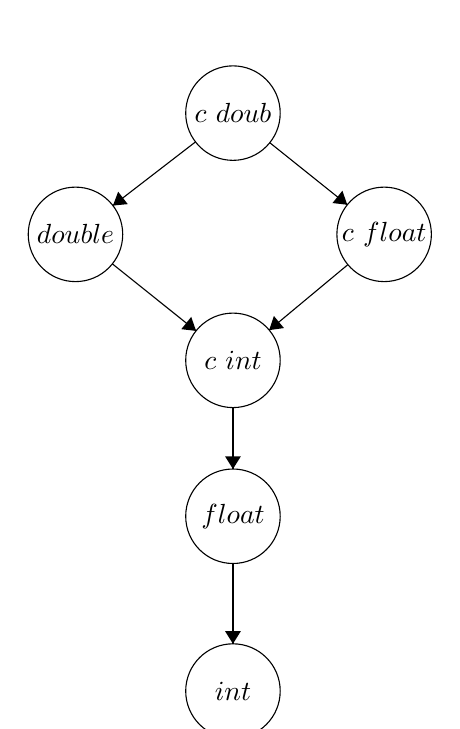
\begin{tikzpicture}[scale=0.2]
\tikzstyle{every node}+=[inner sep=0pt]
\draw [black] (38.5,-46.7) circle (3);
\draw (38.5,-46.7) node {$int$};
\draw [black] (38.5,-35.6) circle (3);
\draw (38.5,-35.6) node {$float$};
\draw [black] (28.5,-17.7) circle (3);
\draw (28.5,-17.7) node {$double$};
\draw [black] (38.5,-25.7) circle (3);
\draw (38.5,-25.7) node {$c\mbox{ }int$};
\draw [black] (38.5,-10) circle (3);
\draw (38.5,-10) node {$c\mbox{ }doub$};
\draw [black] (48.1,-17.7) circle (3);
\draw (48.1,-17.7) node {$c\mbox{ }float$};
\draw [black] (40.84,-11.88) -- (45.76,-15.82);
\fill [black] (45.76,-15.82) -- (45.45,-14.93) -- (44.82,-15.71);
\draw [black] (36.12,-11.83) -- (30.88,-15.87);
\fill [black] (30.88,-15.87) -- (31.82,-15.78) -- (31.21,-14.99);
\draw [black] (38.5,-38.6) -- (38.5,-43.7);
\fill [black] (38.5,-43.7) -- (39,-42.9) -- (38,-42.9);
\draw [black] (45.8,-19.62) -- (40.8,-23.78);
\fill [black] (40.8,-23.78) -- (41.74,-23.65) -- (41.1,-22.88);
\draw [black] (30.84,-19.57) -- (36.16,-23.83);
\fill [black] (36.16,-23.83) -- (35.85,-22.94) -- (35.22,-23.72);
\draw [black] (38.5,-28.7) -- (38.5,-32.6);
\fill [black] (38.5,-32.6) -- (39,-31.8) -- (38,-31.8);
\end{tikzpicture}
\end{center}
%----------------------------------------------------------------------------------------
\end{document}
